\documentclass{article}
\usepackage[preprint]{neurips_2023}
\usepackage[utf8]{inputenc} % allow utf-8 input
\usepackage[T1]{fontenc}    % use 8-bit T1 fonts
\usepackage[ngerman]{babel} % deutsche Silbentrennung und Lokalisierung
\usepackage{hyperref}       % hyperlinks
\usepackage{url}            % simple URL typesetting
\usepackage{booktabs}       % professional-quality tables
\usepackage{amsfonts}       % blackboard math symbols
\usepackage{nicefrac}       % compact symbols for 1/2, etc.
\usepackage{microtype}      % microtypography
\usepackage{xcolor}         % colors
\usepackage{graphicx}
\usepackage[table]{xcolor} % table-Option erlaubt Farbfelder in Tabellen
\usepackage{setspace}
\usepackage{caption} % in die Präambel

% Eigene Farben definieren
\definecolor{Primärblau}{HTML}{45B3CB}
\definecolor{Weiss}{HTML}{FFFFFF}
\definecolor{Schwarz}{HTML}{000000}
\definecolor{Hellgrau}{HTML}{F6F6F6}
\definecolor{Warnorange}{HTML}{FF8000}
\definecolor{Tuerkisgruen}{HTML}{176272}

\onehalfspacing

\title{Documentation Project DISTP}

\author{%
  Group 3 \\
  Otto-Friedrich University Bamberg\\
  Design Interaktiver Systeme in Theorie und Praxis (HCI-DISTP-B) \\ 
  22. August 2025 \\
}


\begin{document}
\maketitle

\begin{abstract}
Diese Dokumentation und Designspezifikation beschreibt die Entwicklung einer medizinischen Anwendung zur kontinuierlichen Überwachung von Vorhofflimmern. Ziel ist es, Patient:innen eine zuverlässige und nutzerfreundliche Lösung bereitzustellen, die frühzeitig Anomalien erkennt und eine effiziente Kommunikation zwischen allen Beteiligten ermöglicht. Die Anwendung integriert Sensordaten, intelligente Algorithmen zur Analyse von Herzrhythmen sowie eine übersichtliche Benutzeroberfläche zur Darstellung relevanter Informationen. Durch den modularen Aufbau ist eine Erweiterung um zusätzliche Diagnose- und Monitoring-Funktionen möglich.
\end{abstract}

\section{Einleitung \& Zielsetzung}
Herz-Kreislauf-Erkrankungen wie Vorhofflimmern gehören zu den häufigsten Ursachen für Schlaganfälle und andere schwerwiegende Komplikationen. Regelmäßige Screenings können Leben retten – doch in der Praxis werden ihre Vorteile oft durch überfordernde Datenmengen, Fehlinterpretationen und die Verunsicherung der Betroffenen gemindert.

Unser Projekt stellt sich dieser Herausforderung mit einer klaren Vision: Eine App, die durch kontinuierliche und smarte Gesundheitsmessungen Sicherheit vermittelt – ohne zu verunsichern – und Ärzten relevante, kontextualisierte Informationen an die Hand gibt, um fundierte Entscheidungen zu erleichtern. Ein ausgemachtes Designziel war es, den Arbeitsaufwand für das medizinische Personal nicht zu erhöhen, da es bereits an der Belastungsgrenze arbeitet. Die App soll sowohl Patienten als auch dem medizinischen Fachpersonal einen spürbaren Mehrwert bieten und dabei ihre individuellen Bedürfnisse berücksichtigen.

\textbf{Für Patienten bedeutet das:}
\begin{itemize}
	\item Einfach zugängliche Messungen von Puls, Blutdruck und EKG über die Smartwatch.
	\item KI-gestützte Unterstützung durch einen Chatbot.
	\item Individuelle Medikamentenpläne und ein optionales Symptomtagebuch.
\end{itemize}

\textbf{Für Ärzte bietet die App:}
\begin{itemize}
	\item Klar aufbereitete, KI-unterstützte Messdaten in einer Reihe von möglichen Formaten.
	\item Zusatzinformationen zu Symptomen und Kontexten aus Patientensicht.
	\item Unterstützung bei der Aufklärung und Beruhigung der Patienten.
\end{itemize}

Unsere Gestaltung folgt den Prinzipien der Offenbacher Produktsprache: Große, selbsterklärende Bedienelemente, beruhigende Farbcodes (Blau als Hauptthema), sanfte Übergänge und eine klare, vertrauenswürdige Typografie. Sicherheit, Verständlichkeit und emotionale Entlastung sind die Kernelemente unseres Designs.

\section{Projektkontext}
\subsection{Unser Team}
Unser Projektteams setzt sich aus einer interdisziplinären Gruppe von Studenten den Universität Bamberg zusammen.

\begin{itemize}
	\item \textbf{Anna Babicheva:} Wirtschaftsinformatik.
	\item \textbf{Hannes Weber:} Angewandte Informatik.
	\item \textbf{Benedikt Freiburg:} Computational Social Science.
	\item \textbf{Peter Geiger:} Computational Social Science.
\end{itemize}

Aufgrund der unterschiedlichen Studienrichtungen bringt jedes Projektmitglied individuelle Perspektiven und Skillsets mit. Da Anna bereits Erfahrungen mit Wireframes aus einem anderen Seminar hatte, übernahm sie die Erstellung der App-Wireframes. Sie war außerdem massgeblich an der konzeptionellen Ausarbeitung der Personas und des Designs beteiligt und wirkte ebenso an dessen praktischen Umsetzung mit. Hannes war für die grundlegenden Designaufgaben verantwortlich und legte damit das Fundament für die spätere Verfeinerung durch Benedikt und Peter. Als technisch versiertestes Mitglied übernahm er zudem die Entwicklung technischer Lösungen für diverse Designprobleme. Benedikt und Peter kümmerten sich um die Detailarbeit, erstellten Screens und setzten Feedback um. 

Für Qualitätssicherung und Barrierefreiheit waren alle Mitglieder gemeinsam zuständig. Eine übergeordnete Projektleitung gab es nicht – wir arbeiteten in einer flachen, hierarchiefreien Struktur. Das verkürzte Kommunikationswege und erleichterte den Feedbackprozess.

\subsection{Projektumfang}
Unsere Kernfeatures belaufen sich auf:
\begin{itemize}
	\item Blutdruck-, Puls- und EKG-Messungen sowie deren Interpretation.
	\item Kontaktfunktion für Angehörige / Notrufoption.
	\item Individuell einstellbare Medikamentenerinnerungen.
	\item Datenexport für Ärzte und Angehörige mit markanten Messwerten, Kontextkommentaren und Verlaufsdarstellung.
	\item Medi-KI-Chat, um schnelle Informationen mittels eines Chatbots zu erhalten und bei einfachen Fragen Ärztinnen und Ärzte zu entlasten.
	\item Möglichkeit für Angehörige, die Werte von Verwandten einzusehen.
	\item Korrespondierende UI für die App auf der Smartwatch.
\end{itemize}

Die sich aus diesen Kernfeatures ableitenden Funktionen sind:
\begin{itemize}
	\item Intuitiver Anmeldescreen.
	\item Datenschutzeinstellungen zur Einhaltung der GDPR.
	\item Verschiedene Abstufungen für Mitteilungen und Benachrichtigungen.
	\item Automatische Messungen zum Erkennen von Mustern im Krankheitsbild.
	\item Erstellung eines Symptomtagebuchs.
	\item Intuitive Sprachauswahl
\end{itemize}

\newpage

\begin{figure}[h!]
	\centering
	\begin{minipage}{0.3\linewidth}
		\centering
		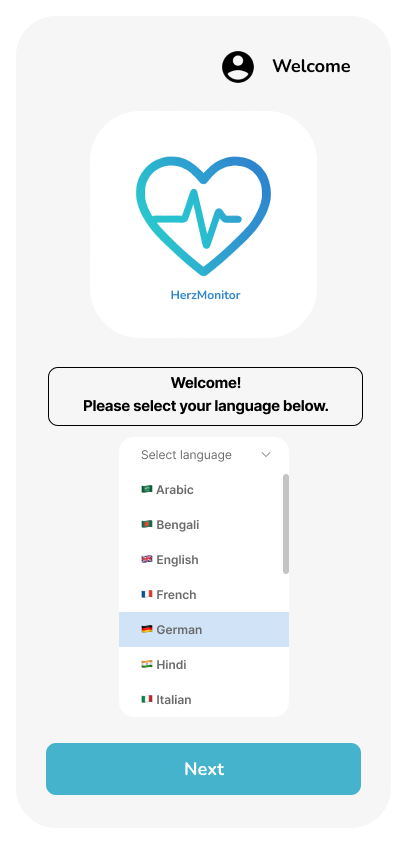
\includegraphics[width=\linewidth]{images/Sprachauswahl}
		\caption{Onboarding: Sprachauswahl}
		\label{fig:sprachauswahl}
	\end{minipage}%
	\hfill
	\begin{minipage}{0.3\linewidth}
		\centering
		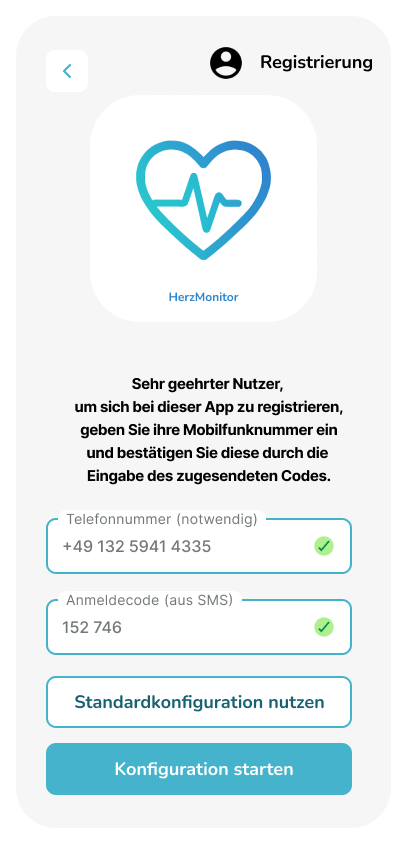
\includegraphics[width=\linewidth]{images/Registrierung}
		\caption{Onboarding: Registrierung}
		\label{fig:registrierung}
\end{minipage}
	\hfill
	\begin{minipage}{0.3\linewidth}
		\centering
		\includegraphics[width=\linewidth]{"images/Homescreen mit Symptomtagebuch"}
		\caption{Hauptmenü mit allen Features}
		\label{fig:homescreen-mit-symptomtagebuch}
	\end{minipage}%
\end{figure}

\vspace{1em}

\subsection{Rahmenbedingungen}
\begin{itemize}
	\item Offenbacher Produktsprache: Grosse, selbsterklärende Buttons, klare visuelle Rückmeldungen, intuitive Navigationslogik, beruhigender Sprachstil.
	\item Sicherheit: Eindeutige Visualisierung von Schutzmechanismen (z.B. Schloss-Icon).
	\item Barrierefreiheit: Klare Kontraste, ausreichend grosse Bedienelemente, einfache Sprache. Möglichkeit, zusätzliche bzw. weiterführende Informationen anzuzeigen, falls dies gewünscht ist.
	\item Styleguide: Farbschema dominiert von Blau (Sicherheit), ergänzt durch Weiss, Hellgrau und sanfte Blautöne. Dieses Farbschema wird nur selten durchbrochen, um z.B. Warnungen wie „Auffälligkeit erkannt“ (\texttt{\#FF8000}, Orange) deutlich darzustellen.
\end{itemize}

\newpage
\section{Designprinzipien}
\subsection{Farbpalette mit Hex-Codes und Verwendungsrichtlinien}

\subsubsection{Primärfarbe}
\begin{itemize}
	\item \textbf{Blau} (\texttt{\#45B3CB}): Hauptbuttons, aktive Navigationselemente, CTAs, Schriften.  
	Blau wurde als Kernthema des Entwurfs gewählt, um den Fokus auf \textbf{Sicherheit} zu betonen. Zudem soll die Farbe beruhigend und schlicht wirken.
\end{itemize}

\subsubsection{Neutralfarben}
\begin{itemize}
	\item \textbf{Blau} (\texttt{\#45B3CB}); \textbf{Weiss} (\texttt{\#FFFFFF}): Haupttext
	\item \textbf{Schwarz} (\texttt{\#000000}): Sekundärtext
	\item \textbf{Hellgrau} (\texttt{\#F6F6F6}): Hintergrundbereiche
\end{itemize}
Auch hier wurde bewusst eine beruhigende Farbpalette eingesetzt. Blau findet sich ebenfalls in den Texten wieder, während Weiß, Schwarz und Hellgrau für Klarheit und Lesbarkeit sorgen.

\subsubsection{Verwendung}
\begin{itemize}
	\item Primärfarben für Interaktionselemente und Überschriften
	\item Neutralfarben für Hintergrund, Text und Layout
\end{itemize}

\subsection{Typografie}

\subsubsection{Schriftarten}
\begin{itemize}
	\item \textbf{Überschriften:} Nunito Bold / Extra Bold
	\item \textbf{Fließtext:} Nunito Regular / Bold
\end{itemize}

\subsubsection{Größen \& Anwendungsbereiche}
\begin{itemize}
	\item \textbf{H1} (\texttt{28--36\,px}): Screen-Titel, Hauptüberschriften
	\item \textbf{Body} (\texttt{20\,px}): Zwischenüberschriften
	\item \textbf{Small} (\texttt{15--18\,px}): Labels, Hilfstexte
\end{itemize}
Auch hier wurde stringent vorgegangen, um die App möglichst übersichtlich und einheitlich zu gestalten.

\newpage

\section{UI-Elemente}
\subsection{Buttons}
\begin{itemize}
	\item \textbf{Primär:} Z.B.\ „Anmelden“, „Speichern“, „Weiter“, „Abbrechen“, „Fertig“.
	\item \textbf{Sekundär:} Z.B.\ „Zurück“, „Erneut erinnern“, „Kommentar speichern“.
	\item \textbf{CTA (Call-to-Action):} Z.B.\ „Notfallkontakt anrufen“, „Medikamentenplan öffnen“.
\end{itemize}

Primäre Buttons sind Blau ausgefüllt (\texttt{\#45B3CB}). Sekundäre Buttons sind nicht ausgefüllt, besitzen jedoch einen blauen Rand (\texttt{\#45B3CB}). Dies signalisiert dem Menschen welcher Button für den weiteren Prozess am wichtigsten ist. Sekundäre Buttons zeigen an, dass hier weitere Funktion und zusätzliche Informationen verfügbar sind.

\subsection{Input-Felder}
\begin{itemize}
	\item Textfelder für Telefonnummern, Codes, Geburtsdaten, Symptombeschreibungen.
	\item Datepicker für Zeit und Datum.
	\item Kommentartextfelder (max. 1000 Zeichen).
\end{itemize}

\subsection{Dropdowns \& Listen}
\begin{itemize}
	\item Dropdowns für Datumsauswahl, Messrhythmus (z.B. täglich, wöchentlich).
	\item Listen für Kontakte, Erinnerungen, Messwerte, Medikation.
\end{itemize}

\begin{figure}[!h]
	\centering
	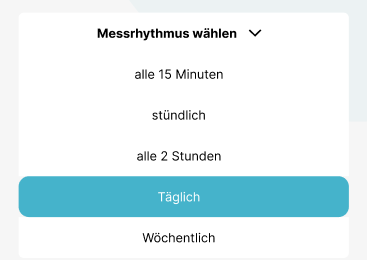
\includegraphics[width=0.45\linewidth]{images/Dropdown}
	\caption{Dropdown-Menü für den Messrhythmus bei Blutdruck \& Puls}
	\label{fig:dropdown}
\end{figure}

\subsection{Navigation}
\begin{itemize}
	\item Hauptmenü mit Modulen wie Erinnerungen, Kontakte, Blutdruck \& Puls, Datenexport, Symptomtagebuch.
	\item Onboarding-Seiten für Registrierung, Einführung, Konfiguration.
\end{itemize}

\subsection{States (Normal, Hover, Disabled, Active)}
\begin{itemize}
	\item \textbf{Normal:} Standardzustand bei Buttons, Eingabefeldern.
	\item \textbf{Disabled:} Buttons ausgegraut, wenn Eingaben fehlen oder Funktion nicht verfügbar ist.
	\item \textbf{Active:} Aktiver Menüpunkt oder laufende Messung (z.\,B.\ Fortschrittsanzeige „30\,\%“).
\end{itemize}

\newpage

\section{User Flows \& Interaktionen}
\subsection{Klickpfade für typische Anwendungsfälle}
Die App hat klare, leicht verständliche Klickpfade für zentrale Anwendungsfälle wie Registrierung, Messungen, Medikamentenerinnerungen und Datenexport. Nutzer werden Schritt für Schritt durch die Abläufe geführt, mit eindeutig, grossen und beschrifteten Buttons sowie konsistenten Bedienelementen.

Die Figma zeigt beispielhaft mehrere Standard-Use-Cases:

\begin{enumerate}
	\item \textbf{Registrierung \& Login}
	\begin{itemize}
		\item Startscreen $\rightarrow$ Sprachauswahl $\rightarrow$ Registrierungsmethode wählen
		\item Telefonnummer/Arztcode eingeben $\rightarrow$ SMS-Code
		\item Profil konfigurieren $\rightarrow$ Weiterführende Informationen $\rightarrow$ Hauptmenü
	\end{itemize}
	
	\item \textbf{Medikamentenplan}
	\begin{itemize}
		\item Hauptmenü $\rightarrow$ Medikamentenplan $\rightarrow$ Erinnerung hinzufügen
		\item Zeit \& Medikament wählen $\rightarrow$ Speichern
	\end{itemize}
	
	\item \textbf{Messungen (Puls/Blutdruck/EKG)}
	\begin{itemize}
		\item Hauptmenü $\rightarrow$ Messung starten $\rightarrow$ Messfortschritt (z.\,B. 30\%)
		\item Ergebnis: „Normal“, „Auffälligkeit erkannt“ oder „Erhöht“
		\item Daten speichern $\rightarrow$ Rückblick/Verlauf
	\end{itemize}
	
	\item \textbf{Datenexport}
	\begin{itemize}
		\item Hauptmenü $\rightarrow$ Datenexport $\rightarrow$ Zeitraum wählen $\rightarrow$ Dateiformat auswählen
		\item Export bestätigen $\rightarrow$ PDF/CSV generieren $\rightarrow$ Download/Teilen
		\item \emph{Alternative:} Hauptmenü $\rightarrow$ Datenexport $\rightarrow$ One-Click Export
	\end{itemize}
	
	\item \textbf{Notfallkontakt hinzufügen}
	\begin{itemize}
		\item Hauptmenü $\rightarrow$ Kontakte $\rightarrow$ „Notfallkontakt hinzufügen“
		\item Telefonnummer eingeben $\rightarrow$ Einladung versenden
		\item Kontakt sichtbar in Liste
	\end{itemize}
	
	\item \textbf{Medi-KI-Chat}
	\begin{itemize}
		\item Hauptmenü $\rightarrow$ Medi-KI-Chat
	\end{itemize}
	
	\item \textbf{Symptomtagebuch}
	\begin{itemize}
		\item Hauptmenü $\rightarrow$ Symptomtagebuch $\rightarrow$ Symptom eintragen $\rightarrow$ Eintrag speichern
	\end{itemize}
\end{enumerate}

\subsection{Feedback-Verhalten (Fehlermeldungen, Bestätigungen)}
Das Feedback-Verhalten nutzt klare Zeichen und Symbole. Meldungen sind präzise formuliert und geben Nutzern sofort verständliche Handlungsempfehlungen.

Die UI zeigt mehrere Interaktionen mit Feedback:
\begin{itemize}
	\item \textbf{Bestätigungen:} „Messung erfolgreich durchgeführt“, „PDF wurde erstellt“
	\item \textbf{Warnungen:} Hinweise bei auffälligen Werten („Vorhofflimmern erkannt“), Medikamentenerinnerungen, Wetterhinweisen etc.
	\item Staffelungen der Warnungen in \textbf{vier Stufen}.
	\item \textbf{Handlungsempfehlungen:} „Bitte wiederholen Sie die Messung in Ruhe“ (häufig in Warnungen integriert), oft auch Hinweise auf Medi-KI-Chat.
\end{itemize}

\newpage

\section{Technische Umsetzung}
Die App setzt auf eine nahtlose Integration zwischen Smartphone und Smartwatch. Die Smartwatch dient als primäre Sensoreinheit für Herzfrequenz-, Blutdruck- oder EKG-Messungen. Über Bluetooth Low Energy (BLE) werden die Daten energieeffizient und in Echtzeit an die App übertragen.
Der Vorteil: Messungen lassen sich auch unterwegs direkt über die Uhr starten, während die App alle Werte automatisch synchronisiert. Ausserdem wird einem Notfallkontakt direkter Zugriff auf die Gesundheitsdaten des Patienten gewährt um so das Sicherheitsgefühl zu erhöhen

\subsection{Hauptfunktionen auf dem Smartphone}
\begin{enumerate}
	\item \textbf{Datenverarbeitung:} 
	Rohdaten werden lokal vorverarbeitet, um Durchschnittswerte, Trends und 
	potenzielle Auffälligkeiten in Echtzeit zu berechnen.
	\item \textbf{Visualisierung:} 
	Messungen werden in Diagrammen dargestellt, inklusive Zeitverläufen und 
	Vergleichswerten.
	\item \textbf{Feedback:} 
	Kritische Werte lösen sofort Warnungen oder Empfehlungen aus, 
	z.B. bei auffälliger Herzfrequenz.
\end{enumerate}

Bei besonders auffälligen Messungen kann automatisch eine Warnung an hinterlegte Angehörige gesendet werden, z. B. per Push-Mitteilung oder SMS.

\begin{figure}[h!]
	\centering
	\includegraphics[width=0.5\linewidth]{images/PulsÜbersicht}
	\caption{Visualisierung des Pulses}
	\label{fig:pulsubersicht}
\end{figure}

\subsection{Sicherheit und Privatsphäre}
\begin{itemize}
	\item \textbf{Ende-zu-Ende-Verschlüsselung:} 
	Alle Messdaten werden verschlüsselt zwischen Smartwatch und Smartphone übertragen.
	\item \textbf{Lokale Speicherung:} 
	Sensible Daten bleiben standardmässig nur auf dem Gerät.
	\item \textbf{Feingranulare Berechtigungen:} 
	Nutzer können gezielt steuern, welche Sensoren oder Funktionen freigegeben werden.
	\item \textbf{Automatische Löschroutinen:} 
	Ältere Daten werden nach einem definierten Zeitraum automatisch entfernt.
\end{itemize}

\subsection{Transparente Kommunikation}
Die App informiert klar über jede Datenerhebung. 
Sicherheitshinweise, Bestätigungsdialoge und optische Marker 
(z.B. ein grünes Schloss-Symbol bei verschlüsselter Verbindung) 
schaffen Vertrauen -- gerade für ältere Nutzer, die besonderen Wert 
auf Datenschutz und einfache Bedienung legen.

\newpage

\section{Personas}
Die Personas wurden in dieser Form aufgebaut, um die verschiedenen Anforderungen, Verhaltensweisen und Erwartungen potenzieller Nutzer:innen unserer App systematisch zu umreißen und verständlich darzulegen. Jede Persona bündelt nicht nur demografische Daten, sondern vor allem Motivationen, Probleme („Pain Points“) und Erwartungen an die App. Dadurch entsteht ein Bild, wie unterschiedliche Zielgruppen mit der App arbeiten und welche Design- und Funktionsentscheidungen daraus erwachsen.

Der Aufbau folgt einem konsistenten Muster: Zunächst wurden Persönlichkeit, Lebensumstände und Interessen dargestellt. So ist ein authentisches, greifbares Bild der Person, das über reine Statistik hinausgeht entstanden. Elemente wie „Was ist in meiner Tasche?“ oder Lieblingsapps helfen, die Personas greifbar zu machen und typische Nutzungssituationen zu demonstrieren. Ebenso geben Abschnitte wie „Freunde \& Familie“ oder „Lebensstil“ Kontext, warum bestimmte Funktionen wichtig sind. So etwa Reminder, um dem Personas in ihrem Alltag zu helfen, oder einfache Bedienbarkeit, wenn wenig Technikaffinität vorhanden ist.

Ein Kernbestandteil ist der Umgang mit der Vorerkrankung. Hier wird deutlich, welche medizinischen Anforderungen gegeben sind und wie sich diese das alltägliche Leben beeinflussen. Daraus lassen sich die spezifischen Aufgaben (z. B. Medikamenteneinnahme, Puls- und Blutdruckkontrolle) sowie die Hauptbedenken der Personas (z.B. Stress, Angst vor Überforderung, falsche Einschätzung durch andere) ableiten. Diese Punkte zeigen, an welchen Stellen die App unterstützen und Sicherheit bieten muss.

Die „Patient Journeys“ bauen darauf auf, indem sie die Lebensabschnitte von den ersten Symptomen bis zur Langzeitbetreuung beschreiben. Jede Phase beinhaltet Gefühle, Verhaltensweisen, Pain Points und Erwartungen. Erkennbar wird so, wie sich die Bedürfnisse im Krankheitsverlauf. Für das Applications-Design ist das von enormer Wichtigkeit, da dies erlaubt, Funktionen angepasst auszurichten: Simple Erklärungen am Anfang, detailreiche Analyse für die Langzeitbetreuung, sowie intuitive Erinnerungen und Benachrichtigungen über den gesamten Zeitraum hinweg.
Zusammenfassend dient dieser Aufbau also dazu, eine Brücke zwischen medizinischen Anforderungen und dem tatsächlichen Alltag der Nutzer:innen zu schlagen. Personas und Patient Journeys machten so die abstrakten Zielgruppen konkret für unser Team erlebbar, deckten Unterschiede (z. B. junge, digitalaffine Nutzerin vs. älterer, technikferner Nutzer) auf und halfen, die App so zu gestalten, dass sie Sicherheit und Vertrauen schafft, Überforderung vermeidet und so hoffentlich langfristig genutzt wird.

\begin{figure}[h!]
	\centering
	\begin{minipage}{0.12\linewidth}
		\centering
		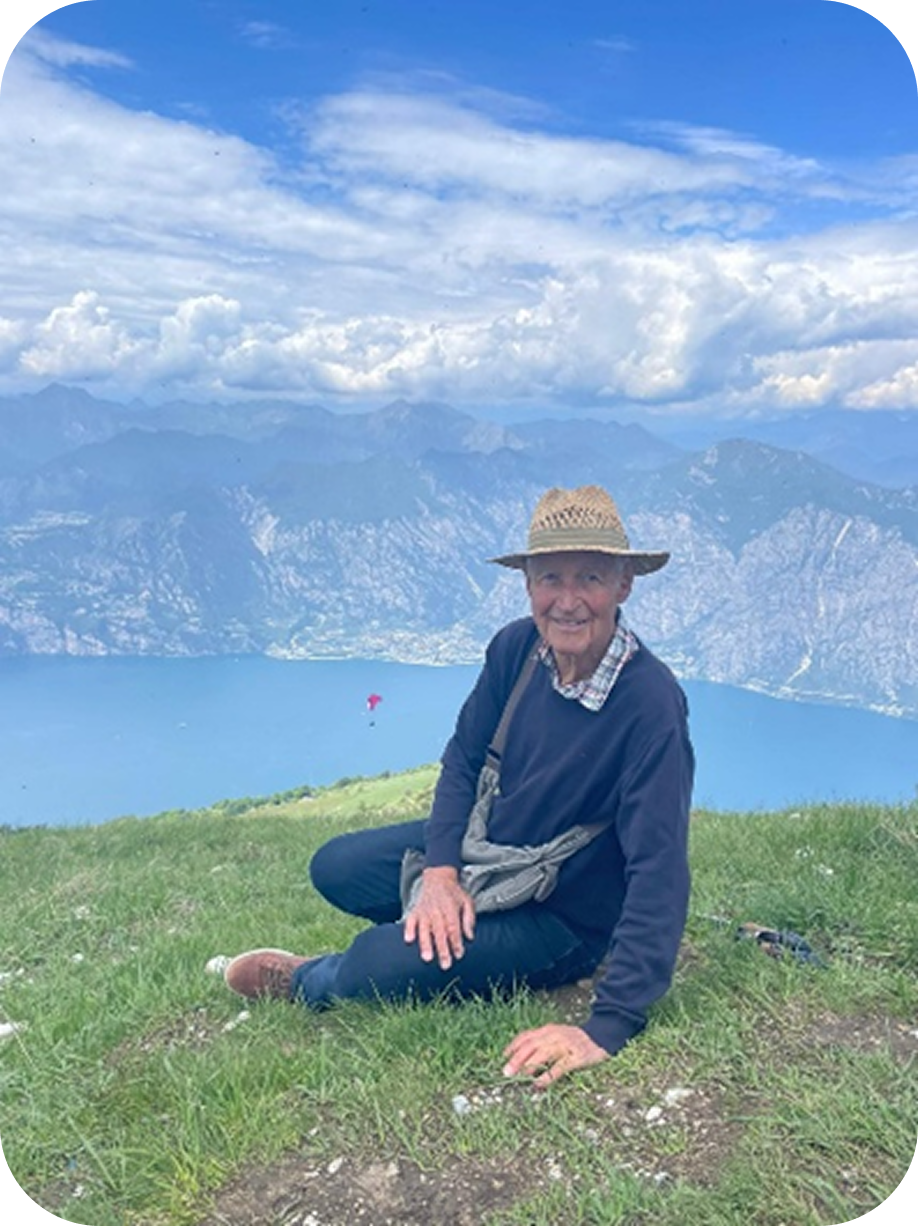
\includegraphics[width=\linewidth]{images/Fred}
		\caption*{Fred Goller}
	\end{minipage}
	\hfill
	\begin{minipage}{0.12\linewidth}
		\centering
		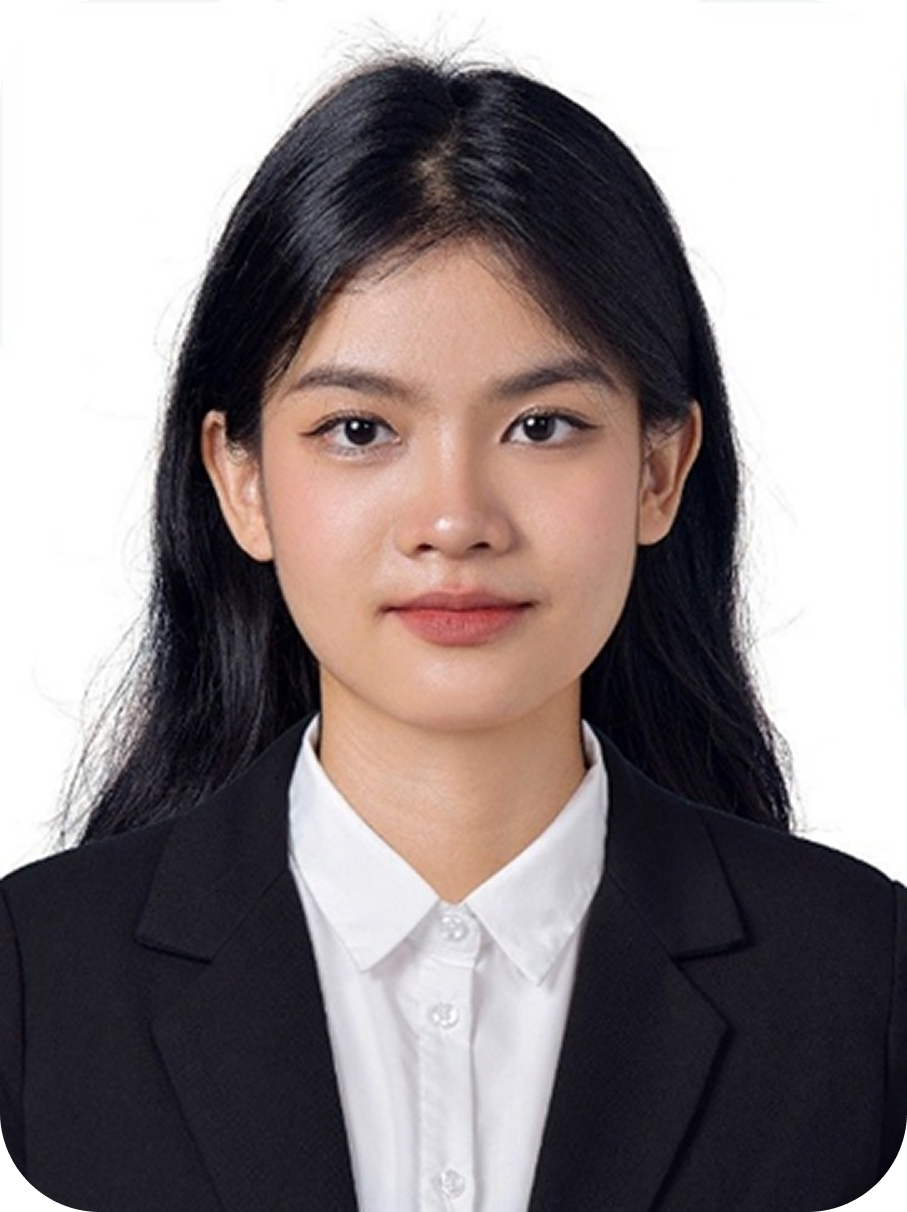
\includegraphics[width=\linewidth]{images/Selina}
		\caption*{Selina Neri}
	\end{minipage}
	\hfill
	\begin{minipage}{0.12\linewidth}
		\centering
		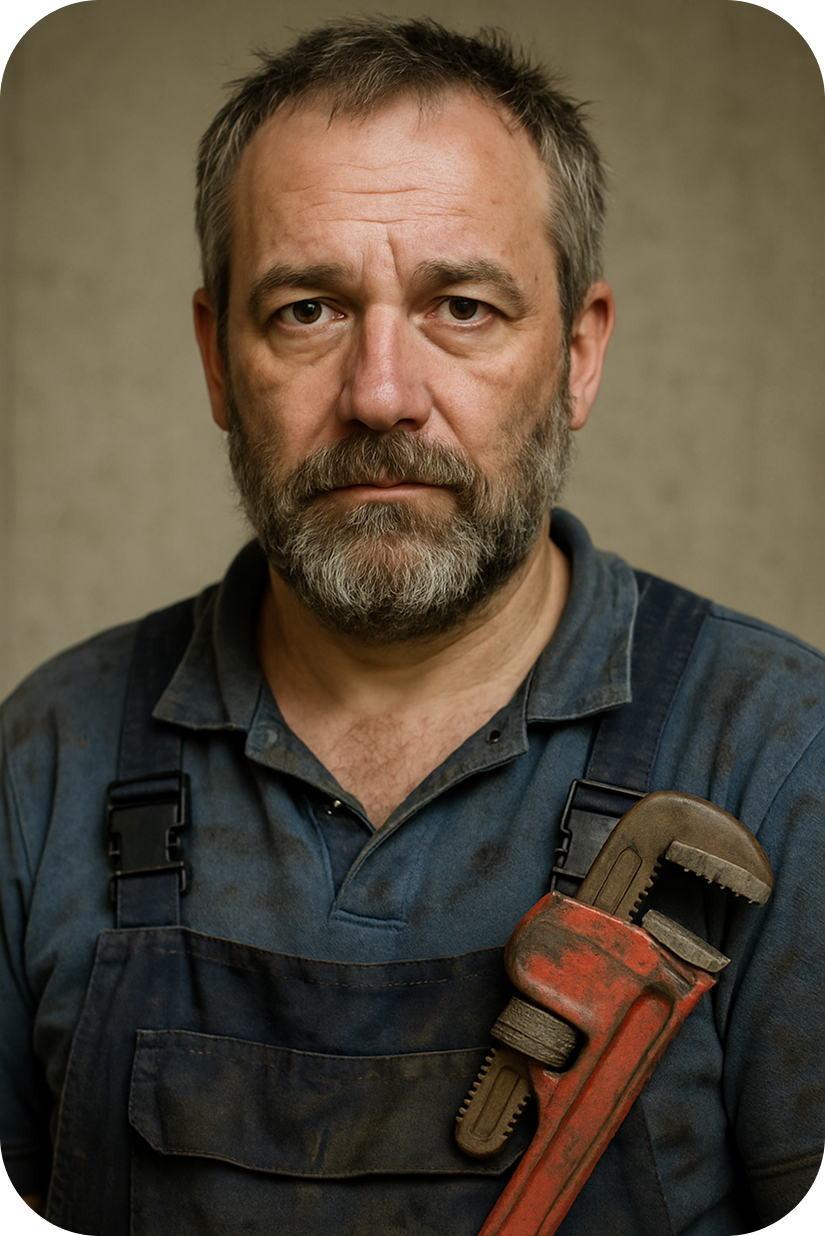
\includegraphics[width=\linewidth]{images/Horst}
		\caption*{Horst Breitenbach}
	\end{minipage}
	\hfill
	\begin{minipage}{0.12\linewidth}
		\centering
		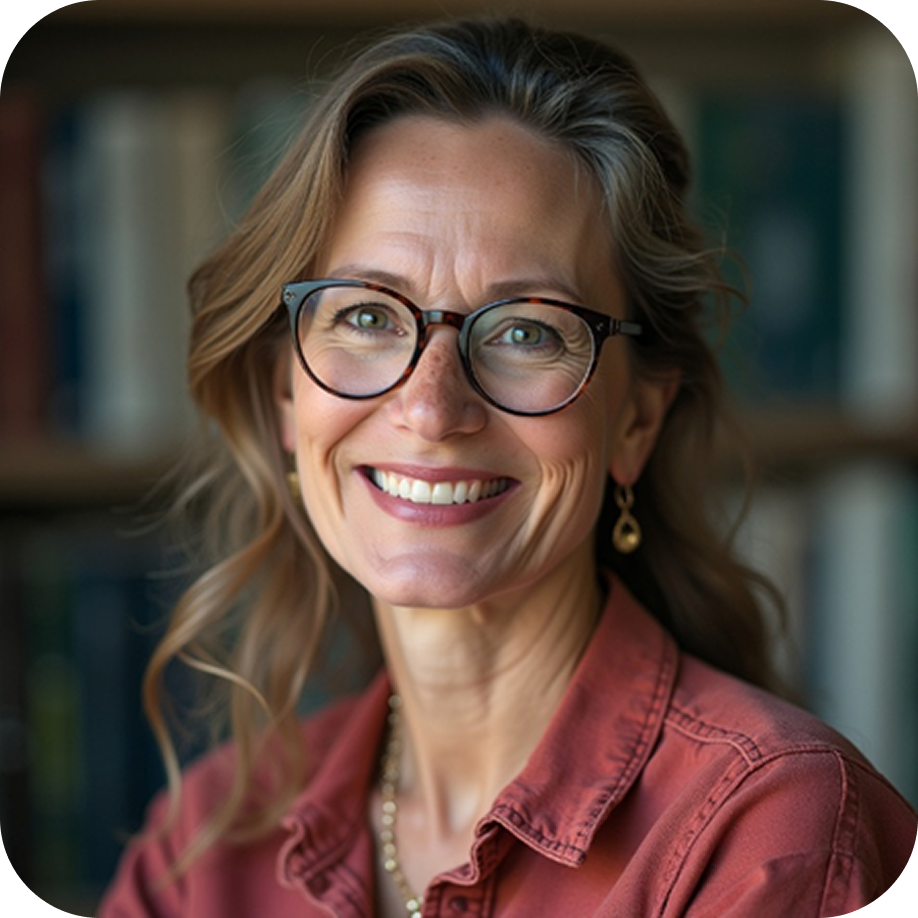
\includegraphics[width=\linewidth]{images/Heike}
		\caption*{Heike Schneider}
	\end{minipage}
	\label{fig:personen}
\end{figure}

\newpage
\section{Journey Map}
\subsection{Ziel der Journey Map}
Die Journey Map dient als generisches Modell des Krankheits- und Betreuungspfades für Patient:innen mit Vorhofflimmern. 
Sie unterteilt die User Experience in vier Hauptphasen. Anschliessend durchläuft die im Projekt definierte Persona jede dieser Phasen 
und bringt unterschiedliche Gefühle, Bedürfnisse und Erwartungen mit. 
All dies trägt zu einem tieferen Verständnis der Prozesse bei.

\subsection{Aufbau}
Die Map wurde in vier Analyseebenen unterteilt:
\begin{itemize}
	\item \textbf{Gefühle und Gedanken} -- emotionale Reaktionen in jeder Phase (z.B. Angst, Vertrauen)
	\item \textbf{Verhalten \& Bedürfnisse} -- welche Handlungen Nutzer:innen typischerweise zeigen (z.B. Arztbesuche, Medikamenteneinnahme)
	\item \textbf{Pain Points} -- kritische Momente, in denen Nutzer:innen besonders gefährdet sind, die App abzulehnen
	\item \textbf{Erwartungen an UI \& App-Funktionalitäten} -- abgeleitete Designanforderungen für jede Phase (z.B. visuelle Sicherheitssignale)
\end{itemize}

\subsection{Phasen}
\begin{description}
	\item[Phase 1: Beginn der Symptome]
	In dieser Phase werden die ersten Anzeichen und Unsicherheiten beschrieben, die die Betroffenen empfinden. 
	Ziel ist es, ihnen Orientierung zu geben und Ängste durch klare und einfache Informationen abzubauen.
	
	\item[Phase 2: Kontakt mit dem Gesundheitssystem \& Diagnose]
	Diese Phase ist den Arztbesuchen, Untersuchungen und der Erstdiagnose gewidmet. 
	Sie zielt darauf ab, Vertrauen aufzubauen und die Patienten bei der Aneignung neuer Gewohnheiten und der Einnahme von Medikamenten zu unterstützen.
	
	\item[Phase 3: Beginn der Behandlung]
	Therapie und regelmässige Messungen werden in dieser Phase Teil des Alltags. 
	Die App soll durch Automatisierung und Vereinfachung der Prozesse dazu beitragen, eine Überlastung zu vermeiden.
	
	\item[Phase 4: Langzeitbetreuung]
	Diese Phase beschreibt eine langfristige Unterstützung, bei der Gesundheit unauffällig in den Alltag integriert wird.
\end{description}
\newpage
\section{Learnings}
Im Verlauf des Projekts konnten wir eine Reihe wertvoller Erkenntnisse gewinnen, die über die Entwicklung des eigentlichen Designs hinausgehen:

\begin{itemize}
	\item \textbf{Bedeutung klarer Kommunikation:} Regelmässige Abstimmungen und die transparente Weitergabe von Informationen haben Missverständnisse reduziert und die Zusammenarbeit gestärkt.
	\item \textbf{Feedback und Sprechstunden:} Generell haben wir gelernt, dass man lieber einmal zu oft als zu wenig nach Feedback fragt. Insgesamt konnte die Anwendung von Feedback unser Produkt merklich verbessern. Konstruktive Kritik wurde als Chance genutzt, die Usability zu steigern und die Bedürfnisse der Personas noch gezielter zu adressieren.
	\item \textbf{Rollenflexibilität:} Die Bereitschaft, auch ausserhalb des eigenen Kernbereichs Aufgaben zu übernehmen, hat den Arbeitsprozess beschleunigt.
	\item \textbf{Feintuning:} Feintuning und Detailarbeit beanspruchen im Design deutlich mehr Zeit als beispielsweise bei Programmieraufgaben.
	\item \textbf{Umgang mit Personas:} Die Personas noch enger in den Designprozess einzubinden, hat zu einem massgeschneiderten Produkt geführt.
\end{itemize}

\newpage


\end{document}
